%%TITLE%%
\title{Does Reuse Survive Reliability? Lifecycle Optimization of Reuse-Based Servers for LLM-Inference Fleets}
%%ABSTRACT%%
\begin{abstract}
Building servers from energy-efficient CPUs and reused DRAM and SSDs cuts the embodied carbon of cloud hardware, but such designs are evaluated at a single point in time, whereas operators decide over years whether to buy, reuse, cascade or retire hardware, and reused parts are already aged and fail more. We formulate a reliability-aware, multi-period lifecycle optimization for large-language-model (LLM) inference fleets that tracks hosts as cohorts by SKU, tier, region and age, precomputes age-dependent failures, repair drains and spare parts from Weibull hazards, couples reuse to a finite supply of harvested parts, allows cascading of previous-generation GPU hosts to a batch tier (in place or to a clean-grid region), and sizes latency-critical reserve with a Monte Carlo chance constraint. On a six-year, three-grid fleet with public and swept parameters, reuse cut lifecycle carbon by 5.77\% on a clean grid but only 0.68\% and 0.10\% on mixed and dirty grids, because operational carbon was about 91\% of a GPU host's lifecycle. A reliability-aware plan retained 0.775\% of a 0.848\% fleet saving and degraded gracefully to zero as reused parts worsened, while a failure-blind plan retained 0.195\% and turned carbon-negative once reused parts failed about 2.1 times more than their age predicts. Guaranteeing a 0.1\% per-region-quarter shortfall probability under strongly correlated failures cost up to 0.82\% extra carbon, and the reuse saving rose to 0.812\% because reused hosts are the cheapest idle reserve. Cascading paid only near energy parity between old and new GPUs. GPU throughput, power and CXL slowdown are placeholders; we provide the measurement methodology to replace them.
\end{abstract}
%%BODY%%
\section{Lifecycle Model}
\label{sec:model}
Figure~\ref{fig:overview} summarizes the model. It answers one question per quarter for every group of identical hosts: keep, retire, cascade, or complement with new or reuse-based hosts and leased capacity, so that demand is met at minimum lifecycle carbon.

\begin{figure}[t]
  \centering
  \includegraphics[width=\linewidth]{figures/fig_lifecycle_model_overview.png}
  \caption{Overview of the reliability-aware lifecycle model. Server SKUs, per-age component reliability, regional grid carbon and demand, and reused-part pools feed a multi-period linear program over fleet cohorts that decides each quarter whether to buy, keep, retire, cascade (in place or to a clean-grid region) or lease capacity. An outer Monte Carlo loop adds latency-critical reserve until every region-quarter meets the target shortfall probability. Outputs are the reuse savings ladder, break-even analyses and the carbon price of a guaranteed SLO.}
  \label{fig:overview}
\end{figure}

\subsection{Fleet State, Decisions and Flow Conservation}
Time is discretized into quarters $t=0,\dots,T-1$ with $T=24$. The fleet is a set of cohorts indexed by SKU $s$, service tier $\tau\in\{\text{LC},\text{BATCH}\}$ (latency-critical and batch inference), region $r$ and node age $a$ in quarters within the node's current life; $n_{s\tau rat}\ge 0$ counts nodes. We model three 8-GPU inference SKUs: \texttt{new\_gpu}, a current-generation host with all-new components; \texttt{green\_gpu}, a reuse-based host in the style of \citet{wang2024greensku} with new GPUs, an energy-efficient CPU, and DRAM (attached over CXL) and SSDs that enter at age $a_0>0$ from a first life; and \texttt{old\_gpu}, a previous-generation host cascaded as a whole from its first life. Cohorts evolve as
\begin{equation}
n_{s\tau rat} = n_{s\tau r,a-1,t-1} - x^{\text{ret}}_{s\tau rat} - [\tau{=}\text{LC}]\sum_{r'} x^{\text{casc}}_{srr'at} + [\tau{=}\text{BATCH}]\sum_{r''} x^{\text{casc}}_{sr''rat} + [a{=}0]\,x^{\text{buy}}_{s\tau rt},
\label{eq:flow}
\end{equation}
with the initial fleet at $t=0$ and forced retirement at a maximum age. A cascade $x^{\text{casc}}_{srr'at}$ moves a node from the LC tier of region $r$ to the BATCH tier of region $r'$ and keeps its age; $r'\neq r$ is \emph{geographic cascading}, which incurs shipping carbon and cost. Building a reuse-based host consumes harvested DIMMs and SSDs from per-component pools, replenished by an external supply (retirements of a general-purpose fleet) and by first-life parts of hosts retired here, after a screening yield of 0.9.

\subsection{Reliability, Capacity and Carbon Accounting}
Each component class $c$ (GPU, CPU, DIMM, SSD) has a Weibull hazard
\begin{equation}
h_c(a)=\frac{k_c}{\eta_c}\left(\frac{a}{\eta_c}\right)^{k_c-1},\qquad H_c(a)=\left(\frac{a}{\eta_c}\right)^{k_c},
\label{eq:weibull}
\end{equation}
whose scale $\eta_c$ is calibrated so that the annual failure probability $1-e^{-(H_c(a^\star+1)-H_c(a^\star))}$ at a reference age $a^\star$ equals an annualized failure rate (AFR). A reused part starts at age $a_0$. A failed part is replaced by a new spare, so each component slot is a delayed renewal process whose first lifetime is conditioned on survival to $a_0$; we solve its renewal equation numerically. Because node age is a cohort index, the expected failures $\lambda_{sa}$, drained hours $d_{sa}$, availability loss $\ell_{sa}=d_{sa}/H$ (with $H$ hours per quarter), and spare and logistics carbon per node-quarter are \emph{precomputed}, and the optimization stays linear. A proportional-hazards multiplier $m$ scales the hazard of reused parts beyond what their age predicts.

Served work $w_{s\tau rat}$, measured in node-equivalents of a fully busy \texttt{new\_gpu} host, obeys
\begin{equation}
w_{s\tau rat}\le n_{s\tau rat}\,\theta_{s\tau}\,u\,(1-\beta_\tau\,\ell_{sa}),
\label{eq:cap}
\end{equation}
where $\theta_{s\tau}$ is relative throughput including the CXL multiplier of the reuse-based host, $u$ the utilization cap and $\beta_\tau$ an LC headroom multiplier ($\beta_{\text{BATCH}}=1$). LC demand $D_{rt}$ is per region; BATCH demand is global. Unserved demand is leased at a carbon premium or counted as shortfall. The objective is lifecycle carbon,
\begin{equation}
C=\sum\Big(e^{\text{emb}}_{sa}n + e^{\text{str}}_{sa}x^{\text{ret}}\Big)+\sum\Big(P^{\text{idle}}_{s}(1-\ell_{sa})H\,n+\kappa_{s\tau}\,w\Big)\,\mathrm{PUE}\cdot\mathrm{CI}_{rt}+\sum\big(q^{\text{sp}}_{sa}+q^{\text{log}}_{sa}\big)n+C^{\text{lease}}+C^{\text{ship}},
\label{eq:obj}
\end{equation}
where embodied carbon $e^{\text{emb}}$ is amortized linearly over the design life and the unamortized remainder $e^{\text{str}}$ is charged on early retirement, operational carbon combines idle power with dynamic energy $\kappa_{s\tau}$ per unit of work, and the grid carbon intensity $\mathrm{CI}_{rt}$ declines per region. Embodied quantities follow component-level accounting in the spirit of architectural carbon models \citep{gupta2022act}. Reused parts carry zero embodied carbon (cut-off accounting) unless stated; we evaluate alternatives in Section~\ref{sec:robust}. Cost and shortfall serve as alternative objectives, and Pareto fronts are traced by $\varepsilon$-constraint. At fleet scale we solve the linear-programming relaxation with HiGHS \citep{huangfu2018highs}.

\subsection{Chance-Constrained SLO Headroom}
Equation~\eqref{eq:cap} protects the LC tier against \emph{expected} drains. An SLO, however, concerns the instantaneous number of drained nodes. With failures arriving at rate $\lambda$ and each repair lasting $d$ hours, the number of drained nodes of a cohort of $N$ nodes is the occupancy of an M/G/$\infty$ queue: Poisson with mean $N\,d_{sa}/H$ for independent failures, or negative binomial with dispersion $k$ for correlated failures (variance $\mu+\mu^2/k$). We add a reserve $R_{rt}$ on \emph{installed} LC capacity,
\begin{equation}
\sum_{s,a}\theta_{s,\text{LC}}\,u\,(1-\beta_{\text{LC}}\ell_{sa})\,n_{s,\text{LC},rat}+\text{lease}_{rt}\ \ge\ D_{rt}+R_{rt},
\label{eq:reserve}
\end{equation}
and iterate: solve; sample instantaneous capacity per region-quarter under the planned fleet; set $R_{rt}\leftarrow R_{rt}+1.05\,\max\{0,\,D_{rt}-Q_\varepsilon(\text{capacity}_{rt})\}$, where $Q_\varepsilon$ is the $\varepsilon$-quantile; re-solve until every gap is at most 0.05\% of demand. Reserves grow monotonically, so the loop terminates; reserve nodes are idle and therefore pay idle power and embodied carbon, which is the carbon price of the SLO. Final plans are validated by an independent replay with 50{,}000 samples.

\section{Evaluation Methodology}
\label{sec:method}
\subsection{Scenarios and Parameters}
\emph{Node level:} one host per SKU over a six-year life at 60\% utilization on three grids with base carbon intensity 40, 250 and 650\,gCO$_2$e/kWh (clean, mixed, dirty) declining 2\%, 5\% and 3\% per year, and PUE 1.2. \emph{Reference fleet:} 24 quarters and three regions; LC demand starts at 180, 450 and 330 node-equivalents (clean, mixed, dirty) and grows 25\%, 25\% and 30\% per year; global BATCH demand starts at 150 and grows 35\% per year. The initial fleet holds about 1{,}750 hosts: 150/500/400 previous-generation hosts and 100/350/250 current-generation hosts per region. Reused-part pools start with 3{,}200 DIMMs and 800 SSDs and receive 2{,}400 DIMMs and 600 SSDs per quarter.

Per-unit embodied carbon is 150\,kgCO$_2$e for a current-generation GPU, 120 for a previous-generation GPU, 30 for a CPU, 20 for a 64\,GB DIMM and 614 for a 3.84\,TB SSD; \texttt{new\_gpu} draws 2{,}500\,W idle and 10{,}200\,W peak. Weibull shapes and AFRs are 1.0/0.0868 (GPU), 1.0/0.002 (CPU), 1.6/0.01 (DIMM) and 1.3/0.01 (SSD), with drains of 72, 24, 8 and 2 hours per failure. The GPU AFR is derived from a published interruption report of a 54-day pretraining run on about 16{,}384 GPUs with 148 faulty-GPU and 72 GPU-memory interruptions \citep{llama3}. All other parameters are engineering assumptions with ranges that we sweep. \textbf{GPU throughput, power and the CXL slowdown are placeholders} (relative throughput of \texttt{old\_gpu} 0.30 LC and 0.45 BATCH; CXL multiplier 0.95 LC and 0.98 BATCH); results that depend on them are model-based. No proprietary fleet data is used.

\subsection{Experiment Ladder, Metrics and Solver}
We compare plans on the same scenario. E0: no reuse (only new hardware), with failures ignored (E0$_\text{det}$) or counted. E1: reuse allowed, failures ignored. E2a: E1's purchase and retirement decisions replayed with failures. E2b: reuse with a reliability-aware plan. E3/E3g: E2b plus in-place / geographic cascading. Savings are $X=1-C(\text{E1})/C(\text{E0}_\text{det})$, $Y_\text{naive}=1-C(\text{E2a})/C(\text{E0})$, $Y=1-C(\text{E2b})/C(\text{E0})$, and $Z$ ($Z_g$) is the additional saving of E3 (E3g) over E2b in percentage points.

The mixed-integer formulation of a 36-node pilot hit a 300\,s limit without proving optimality, while its LP relaxation solved in under 1\,s, matched the integer $X$ and $Y$ within about 0.05 percentage points, and gave identical results at 1$\times$ and 50$\times$ fleet scale; all fleet results therefore use the relaxation, and a full ladder solves in about 4\,s. A suite of 40 tests, including a hand-calculated single-SKU case, passes.

We also prepared, but have not yet executed, three GPU measurements to replace the placeholders: a serving benchmark on a paged-KV-cache serving engine \citep{kwon2023vllm} that measures LC goodput under time-to-first-token and time-per-output-token SLOs and BATCH throughput with board power (tokens per joule) per GPU generation; a KV-cache offload benchmark with the cache in local versus remote-NUMA host memory as a proxy for CXL-attached reused DRAM; and KV-cache fault injection at controlled bit-error rates under no protection, SECDED ECC and block checksums with recomputation.

\section{Results}
\label{sec:results}
\subsection{Operational Carbon Dominates GPU Hosts}
Table~\ref{tab:node} gives six-year node-level carbon on the mixed grid. Operational carbon was about 91\% of a new host's lifecycle carbon. Reuse cut the host's embodied carbon by about two thirds, from 8{,}312 to 2{,}860\,kgCO$_2$e, but changed its total by only about 6\%. Per unit of work, the reuse-based host saved 18.23\% (LC) and 20.73\% (BATCH) on the clean grid, 1.26\% and 4.28\% on the mixed grid, and $-2.04\%$ and 1.08\% on the dirty grid with failures ignored; counting failures lowered these by 0.1 to 2.2 percentage points. The sign on the mixed grid hinged on the CXL throughput multiplier, whose range of 0.85--1.0 moved the saving from $-10.72\%$ to 5.88\%, a swing of 16.61 percentage points---three times the next parameter, the reuse host's peak-power delta (5.65), followed by SSD embodied carbon (5.41) and grid carbon intensity (4.20) (Figure~\ref{fig:tornado}).

\begin{table}[t]
  \centering
  \caption{Six-year lifecycle carbon per node (kgCO$_2$e), mixed grid, LC tier, failures counted.}
  \label{tab:node}
  \begin{tabular}{lrrrrr}
    \toprule
    SKU & Embodied & Operational & Spares + logistics & Total $\downarrow$ & Failures/node \\
    \midrule
    \texttt{new\_gpu} & 8{,}312 & 96{,}662 & 1{,}291 & 106{,}265 & 10.62 \\
    \texttt{green\_gpu} & 2{,}860 & 95{,}511 & 1{,}575 & 99{,}945 & 15.18 \\
    \texttt{old\_gpu} & 0 & 62{,}344 & 1{,}896 & 64{,}240 & 18.42 \\
    \bottomrule
  \end{tabular}
\end{table}

\begin{figure}[t]
  \centering
  \includegraphics[width=0.85\linewidth]{figures/fig_node_sensitivity_tornado.png}
  \caption{One-at-a-time sensitivity of the node-level reuse saving (mixed grid, latency-critical tier) to each parameter's range. Bars show the saving with the parameter at the low (blue) and high (orange) ends; the CXL throughput multiplier alone determines the sign of the saving.}
  \label{fig:tornado}
\end{figure}

\subsection{Does Reuse Survive Reliability?}
Table~\ref{tab:ladder} and Figure~\ref{fig:ladder} report the fleet ladder. Ignoring failures, reuse saved $X=0.848\%$. A reliability-aware plan kept $Y=0.775\%$, about 91\% of it. A failure-blind plan kept only $Y_\text{naive}=0.195\%$: it purchased the same reuse-heavy fleet as E1, then had to lease 13{,}104\,tCO$_2$e of capacity to cover drained nodes, against 530\,tCO$_2$e for the reliability-aware plan. Split by grid, $X$ was 5.766\%, 0.675\% and 0.103\% and $Y$ was 5.028\%, 0.568\% and 0.087\% on clean, mixed and dirty single-grid fleets, while the failure-blind plan saved 4.584\% and 0.039\% on clean and mixed grids and lost 0.443\% on the dirty grid.

\begin{table}[t]
  \centering
  \caption{Reference fleet: six-year lifecycle carbon by plan (tCO$_2$e).}
  \label{tab:ladder}
  \begin{tabular}{lrrrrr}
    \toprule
    Plan & Total $\downarrow$ & Embodied & Operational & Spares + log. & Leased \\
    \midrule
    E0$_\text{det}$: no reuse, failures ignored & 484{,}413 & 24{,}134 & 460{,}279 & 0 & 0 \\
    E0: no reuse, failures counted & 490{,}607 & 24{,}606 & 462{,}068 & 3{,}933 & 0 \\
    E1: reuse, failures ignored & 480{,}305 & 18{,}871 & 460{,}937 & 0 & 497 \\
    E2a: failure-blind plan, replayed & 489{,}652 & 18{,}871 & 453{,}457 & 4{,}220 & 13{,}104 \\
    E2b: reliability-aware reuse & 486{,}804 & 19{,}716 & 462{,}295 & 4{,}264 & 530 \\
    E3: E2b + cascading & 486{,}780 & 19{,}715 & 462{,}574 & 4{,}301 & 191 \\
    \bottomrule
  \end{tabular}
\end{table}

\begin{figure}[t]
  \centering
  \includegraphics[width=\linewidth]{figures/fig_fleet_carbon_ladder_by_grid.png}
  \caption{Left: change in six-year lifecycle carbon relative to the no-reuse fleet, by carbon component, for a failure-blind reuse plan, a reliability-aware reuse plan, and the latter with in-place or geographic cascading; dots mark the net change. Right: reuse savings $X$ (failures ignored), failure-blind, $Y$ (reliability-aware) and $Y$ plus cascading for single-grid fleets on clean, mixed and dirty grids. GPU throughput, power and CXL slowdown are placeholder values.}
  \label{fig:ladder}
\end{figure}

Figure~\ref{fig:reliab} sweeps the reused-part hazard multiplier $m$. The reliability-aware plan bought fewer reuse-based hosts as $m$ grew, with $Y$ falling from 0.863\% ($m=0.5$) to 0.621\% ($m=2$), 0.209\% ($m=5$) and 0 from $m=8$ onwards; it never chose a plan worse than no reuse. The failure-blind plan crossed zero near $m\approx2.1$ and reached $-2.251\%$ at $m=20$. At node level, the aged DIMMs nearly doubled DIMM failures (9.67 against 5.43 per host over six years), but each DIMM swap drains 8\,h whereas GPU failures, common to both SKUs, drain 72\,h; GPU failures therefore dominated drained hours (394 against 359\,h per host in total), which is why reliability eroded savings mainly through planning rather than through raw failure counts.

\begin{figure}[t]
  \centering
  \includegraphics[width=0.75\linewidth]{figures/fig_reliability_breakeven_reused_parts.png}
  \caption{Fleet carbon saving of reuse versus a multiplier on reused-part failure rates beyond the age effect. The reliability-aware plan degrades gracefully and stops reusing at a multiplier of about 8, never doing worse than no reuse; a plan that ignores failures crosses zero near 2 and becomes increasingly carbon-negative.}
  \label{fig:reliab}
\end{figure}

\subsection{When Does Cascading Pay?}
Cascading added essentially nothing at the placeholder efficiency ($Z=0.005$ percentage points; old/new BATCH work per joule 0.70). Figure~\ref{fig:cascade} sweeps that ratio. $Z$ stayed at or below 0.027 points up to a ratio of 0.935, then rose to 0.109 (ratio 1.168) and 0.346 (ratio 1.869). Above parity, geographic cascading to the clean region's BATCH tier added roughly 50--70\% on top ($Z_g=0.184$ and 0.521 at ratios 1.168 and 1.869). Because cascading avoids only the embodied carbon of new hosts, which is a small share of a GPU host's lifecycle, it cannot compensate for an operational-efficiency gap.

\begin{figure}[t]
  \centering
  \includegraphics[width=0.75\linewidth]{figures/fig_cascade_breakeven_energy_efficiency.png}
  \caption{Additional carbon saving from cascading previous-generation GPU hosts to the batch tier versus their batch work per joule relative to current-generation hosts. Cascading pays only near energy parity; shipping cascaded hosts to the clean-grid region adds further savings once cascading pays.}
  \label{fig:cascade}
\end{figure}

\subsection{Guaranteeing the SLO}
Replaying the expected-value plans (headroom multiplier 3) against sampled drains showed that the LC tier met demand on average but not everywhere: the worst region-quarter had a 2.7\% probability of LC shortfall without reuse and 14.5\% with reliability-aware reuse under independent failures, rising to 15.5\% under correlated failures; under strong correlation ($k=0.5$), 44--48 of 72 region-quarters exceeded 1\%. Table~\ref{tab:slo} and Figure~\ref{fig:slo} report the chance-constrained plans. Every plan met its target in independent validation (worst region-quarter 1.00--1.07\% for a 1\% target and 0.10--0.13\% for 0.1\%), converging in 4 to 15 iterations. The SLO cost 0.22--0.82\% extra carbon, rising with strictness and correlation; strongly correlated failures required about 2.6$\times$ the reserve of independent ones at the 0.1\% target. In every setting the reuse plan paid a slightly lower price than the no-reuse plan, so the reuse saving \emph{grew} under the guarantee: from 0.775\% to 0.812\%, and from 0.480\% to 0.500\% when reused parts failed three times more than their age predicts.

\begin{table}[t]
  \centering
  \caption{Chance-constrained LC headroom: reuse saving $Y$ under a guaranteed SLO and the carbon price of the SLO, both in \%. $m$ is the reused-part failure multiplier and $\varepsilon$ the per-region-quarter shortfall target.}
  \label{tab:slo}
  \begin{tabular}{rlrrrrr}
    \toprule
    $m$ & Correlation & $\varepsilon$ & $Y$ guaranteed $\uparrow$ & $Y$ expected & Price (reuse) & Price (no reuse) \\
    \midrule
    1 & independent & 0.01 & 0.786 & 0.775 & 0.217 & 0.229 \\
    1 & independent & 0.001 & 0.788 & 0.775 & 0.301 & 0.314 \\
    1 & $k=2$ & 0.001 & 0.792 & 0.775 & 0.427 & 0.445 \\
    1 & $k=0.5$ & 0.01 & 0.795 & 0.775 & 0.477 & 0.497 \\
    1 & $k=0.5$ & 0.001 & 0.812 & 0.775 & 0.785 & 0.823 \\
    3 & independent & 0.001 & 0.484 & 0.480 & 0.310 & 0.314 \\
    3 & $k=0.5$ & 0.001 & 0.500 & 0.480 & 0.803 & 0.823 \\
    \bottomrule
  \end{tabular}
\end{table}

\begin{figure}[t]
  \centering
  \includegraphics[width=\linewidth]{figures/fig_chance_constrained_slo.png}
  \caption{Left: reuse saving under a guaranteed latency-critical SLO (per region-quarter shortfall probability of at most 1\% or 0.1\%) for independent and increasingly correlated failures, with reused parts failing as their age predicts (1$\times$) or three times more (3$\times$). Right: carbon price of the SLO for the reuse plan relative to its expected-value plan.}
  \label{fig:slo}
\end{figure}

\subsection{Robustness: Accounting, Uncertainty, Headroom and Cost}
\label{sec:robust}
\emph{Accounting.} The convention for reused parts changed magnitudes but not rankings (Table~\ref{tab:robust}): $Y$ was 0.775\% with cut-off and amortized accounting, 0.601\% when reused parts carried their unamortized share, 1.423\% and 1.067\% with upfront accounting, and 0 when reused parts were charged as new, in which case the failure-blind plan lost 0.506--0.557\%. \emph{Fuzzy uncertainty.} With triangular factors on failure rates $\times[0.5,1,3]$, embodied carbon $\times[0.5,1,2]$ and the CXL multiplier $[0.85,0.95,1.0]$, propagated by $\alpha$-cuts \citep{zadeh1965fuzzy} as in multi-objective fuzzy circular-economy models \citep{poonia2024circular}, $Y$ lay in $[0.000,2.638]\%$ at $\alpha=0$ and $[0.266,1.489]\%$ at $\alpha=0.5$; the lower bound never fell below zero and the upper bound was driven mainly by embodied carbon. \emph{Utilization and headroom.} $Y$ was higher at a 0.5 utilization cap (0.783--0.806\%) than at 0.8 (0.775--0.777\%), consistent with embodied carbon mattering more on lightly loaded capacity; the share of node-quarters on reuse-based hosts fell from 0.303 to 0.280 as the LC headroom multiplier rose from 1 to 10. \emph{Cost.} The cost-minimal plan emitted 499.5\,ktCO$_2$e at USD 1.437 billion and the carbon-minimal plan 486.8\,ktCO$_2$e at USD 1.719 billion: 2.6\% more carbon for 16\% less cost, with most of the carbon gain available within about 5\% extra cost (Figure~\ref{fig:pareto}).

\begin{table}[t]
  \centering
  \caption{Reuse savings (\%) under embodied-carbon accounting conventions for reused parts.}
  \label{tab:robust}
  \begin{tabular}{llrrr}
    \toprule
    Reused-part charge & Amortization & $X$ & $Y_\text{naive}$ & $Y$ \\
    \midrule
    cut-off (zero) & amortized & 0.848 & 0.195 & 0.775 \\
    cut-off (zero) & upfront & 1.544 & 0.918 & 1.423 \\
    residual share & amortized & 0.667 & 0.029 & 0.601 \\
    residual share & upfront & 1.181 & 0.562 & 1.067 \\
    charged as new & amortized & 0.000 & $-0.557$ & 0.000 \\
    charged as new & upfront & 0.000 & $-0.506$ & 0.000 \\
    \bottomrule
  \end{tabular}
\end{table}

\begin{figure}[t]
  \centering
  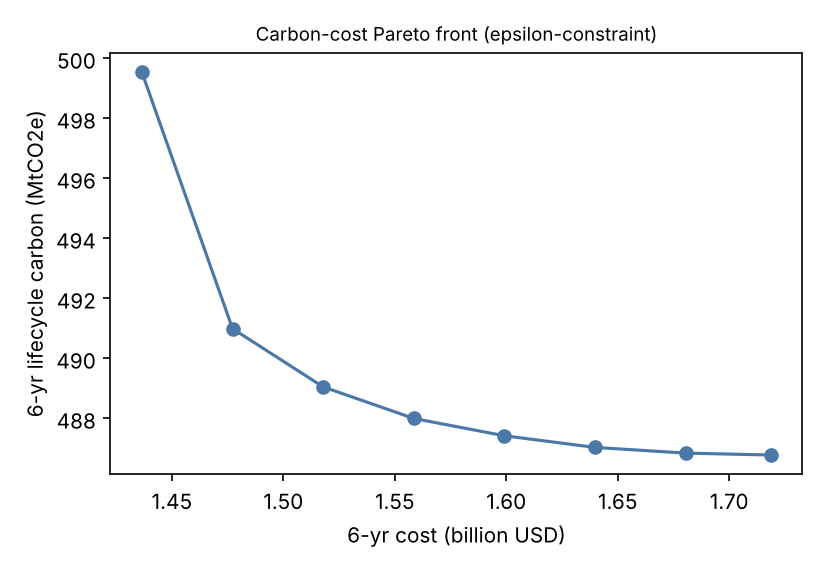
\includegraphics[width=0.7\linewidth]{figures/p3_pareto.png}
  \caption{Carbon--cost $\varepsilon$-constraint front of the reference fleet over six years.}
  \label{fig:pareto}
\end{figure}

\section{Discussion and Limitations}
\label{sec:discussion}
\subsection{Design Implications}
Three implications follow for reliability-aware reuse in AI fleets. First, place reuse where it pays: reuse-based hosts belong in clean-grid regions and in reserve or lightly loaded capacity, where embodied carbon dominates, while steadily loaded capacity on carbon-intensive grids is best served by the most energy-efficient hosts. Second, plan for reliability rather than ignoring it: the same reuse decision is beneficial under a reliability-aware plan and harmful under a failure-blind one, so lifecycle planners must carry per-age failure, drain and spare models. Third, treat cascading old GPUs as a cost lever unless their batch energy efficiency approaches parity with new GPUs; if it does, ship them to clean grids.

\subsection{Limitations}
Our conclusions are bounded by the modelling setting. GPU throughput, power and the CXL slowdown are placeholders; the cascading verdict and the sign of reuse savings on mixed grids depend on them, which is why we provide the measurement methodology of Section~\ref{sec:method}. Except for the GPU failure rate, embodied-carbon and failure parameters are assumptions whose ranges we sweep. Reliability enters the LP as expected values, with tail behaviour handled by the outer Monte Carlo loop rather than inside the optimization, and fleet results use the LP relaxation. The study uses no proprietary fleet data.

\section{Conclusion}
\label{sec:conclusion}
We asked whether the carbon savings of server component reuse survive the reliability of aged, reused parts in LLM-inference fleets. A reliability-aware lifecycle optimization answers in three parts: the grid sets the magnitude of reuse savings; reuse survives reliability when planning accounts for it and fails when it does not; and reuse persists---slightly strengthened---under guaranteed SLOs because reused hosts are the cheapest idle reserve. Executing the prepared GPU measurements is the next step to replace the remaining placeholders.
